\section{Existing Multi-Error Tolerant Designs} \label{sec:DNUdes}

In this section, we discuss the existing DNU tolerant designs and give a background for the TNU latch. First we will discuss the DNU tolerant designs. The first proposed design, designated as the DNCS (Double Node Charge Sharing) latch is presented in \cite{DNCS} and Fig. \ref{DNCS_fig}. It contains two DICE latches connected to a 2-input C-element. The DICE latch consists of 4 one-input c-elements connected in series. Two of the nodes are connected to a pass-gate which allows data to be loaded. Additionally, an example of the C-element is given in Fig. \ref{Cele_fig}. The idea behind this design that it is impossible for a DNU to flip both DICE latches since they are SEU tolerant. More specifically, since the DICE latch is SEU tolerant, it requires a DNU to upset the data on a single cell. Even if a single cell is upset, the output C-element will hold the correct state. The output C-element only changes value when the inputs are unanimously the same value. Since both latches cannot be upset, the DNCS will tolerate a DNU. While this design is DNU tolerant, it is not DNU-robust since it may move to a high-impedance state after an error. 

\begin{figure}[!htbp]
	\centering
	%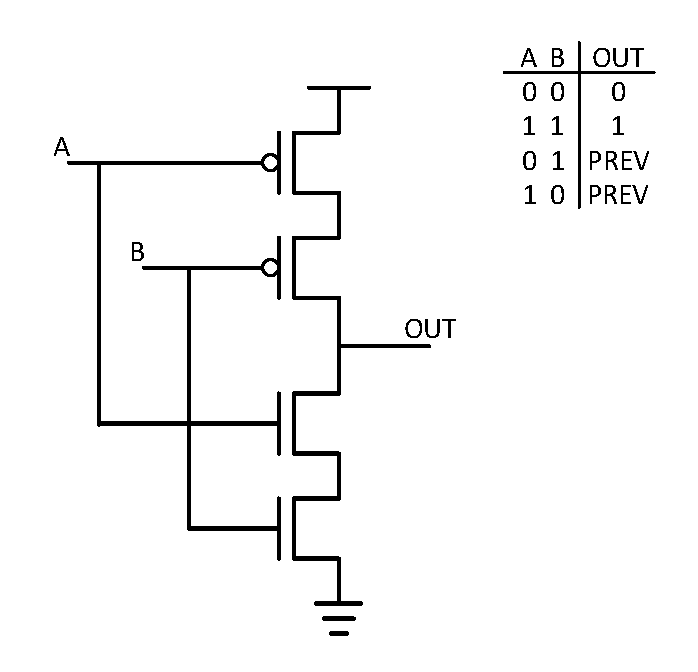
\includegraphics[width=0.55\linewidth]{Figures/C_ele}
	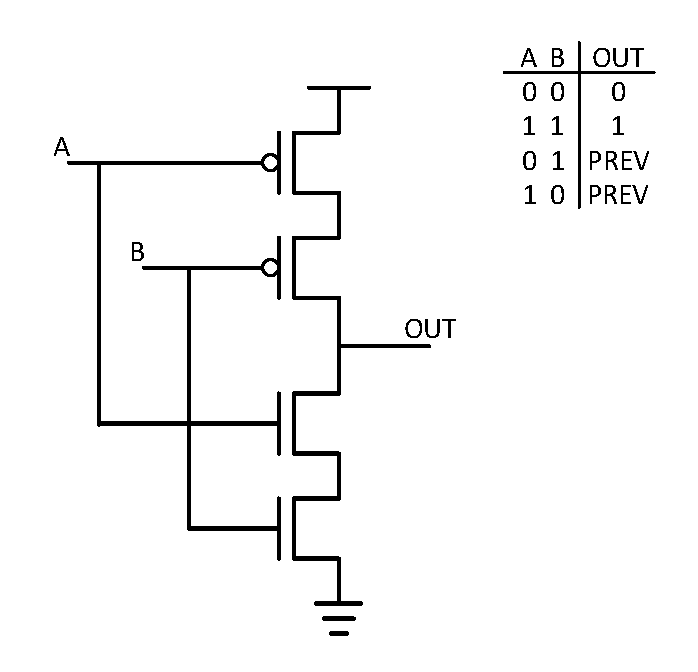
\includegraphics[trim = 0mm 6mm 0mm 7mm, clip, width=0.55\linewidth]{Figures/C_ele}	
	%where an .eps filename suffix will be assumed under latex, 
	%and a .pdf suffix will be assumed for pdflatex; or what has been declared
	%via \DeclareGraphicsExtensions.
	\caption{Muller C-element}
	\label{Cele_fig}
\end{figure}

\begin{figure}[!htbp]
	\centering
	%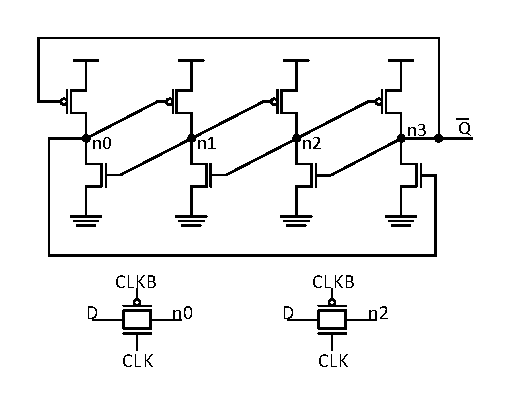
\includegraphics[width=0.8\linewidth]{Figures/DICE}
	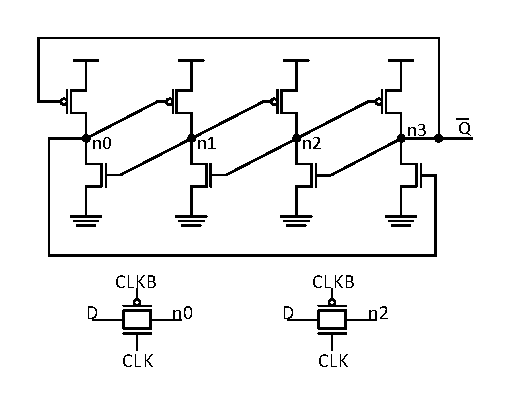
\includegraphics[trim = 0mm 6mm 0mm 6mm, clip, width=0.8\linewidth]{Figures/DICE}
	%where an .eps filename suffix will be assumed under latex, 
	%and a .pdf suffix will be assumed for pdflatex; or what has been declared
	%via \DeclareGraphicsExtensions.
	\caption{DICE Latch.}
	\label{DICE_fig}
\end{figure}

\begin{figure}[!htbp]
	\centering
	%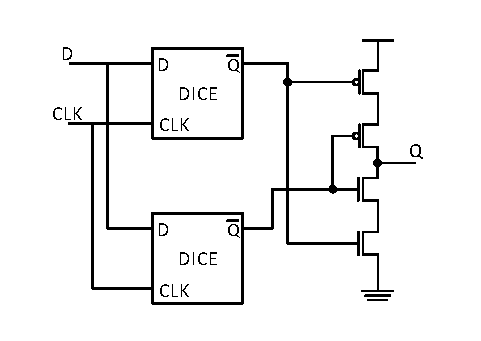
\includegraphics[width=0.8\linewidth]{Figures/DNCS}
	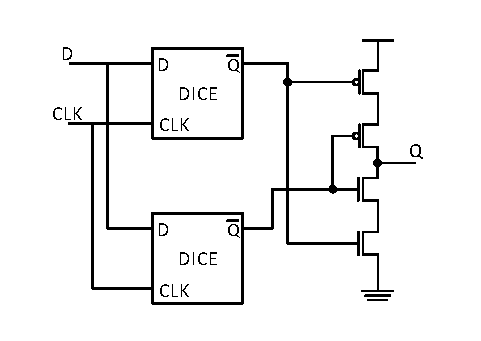
\includegraphics[trim = 0mm 6mm 0mm 7mm, clip, width=0.8\linewidth]{Figures/DNCS}
	%where an .eps filename suffix will be assumed under latex, 
	%and a .pdf suffix will be assumed for pdflatex; or what has been declared
	%via \DeclareGraphicsExtensions.
	\caption{The DNCS latch. A diagram of the DICE latch is given in Fig. \ref{DICE_fig}.}
	\label{DNCS_fig}
\end{figure}

Another design, named the interception latch and proposed in \cite{Inter}, improves on the DNCS by providing lower power consumption, delay and area. The latch functions using six 2-input C-elements connected in series. Every other node in the latch is fed to an output 3-input C-element. In this design, a DNU can only flip at most two nodes. Since the output is voted on by a C-element, it will not change value. Like the DNCS latch, a DNU will force the latch into a high-impedance state which implies the latch is DNU non-robust.

The most recent and efficient DNU tolerant latch is the HSMUF which is proposed in \cite{HSMUF} and illustrated in Fig. \ref{HSMUF_fig}. This latch uses the TP-DICE structure found in \cite{TPDICE}. It is an extended DICE cell with a total of 6 nodes. In the TP-DICE cell, every other node is connected to the input of a 3-input Muller C-element. When a DNU occurs in the worst case, two nodes are set to erroneous value, two nodes are set to high-impedance and two nodes hold the correct value. Since a Muller C-element is placed on the output, the high-impedance and error-free nodes hold the output to the correct value. However, a drawback with this design is that it relies on high impedance states for reliability thus the design is non-robust. A common way to mitigate this issue is to place a weak-keeper at the output of the latch as in Fig. \ref{HSMUF_fig}. While this design does ensure the output is held, the C-element must be sized such that the driving strength exceeds that of the keeper. According to our simulations found in Section \ref{sec:res}, the addition of the keeper substantially increases the delay, area and power consumption. 

\begin{figure}[!htbp]
\centering
%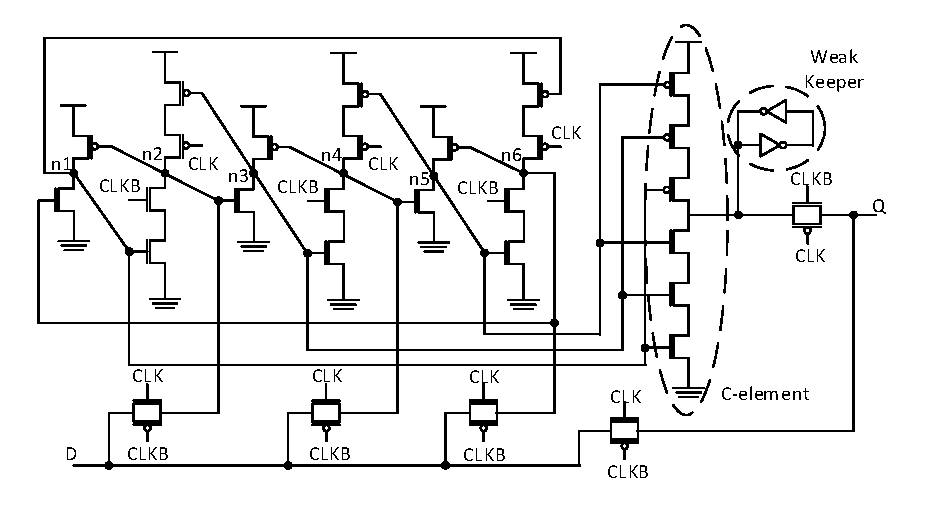
\includegraphics[width=\linewidth]{Figures/HSMUF}
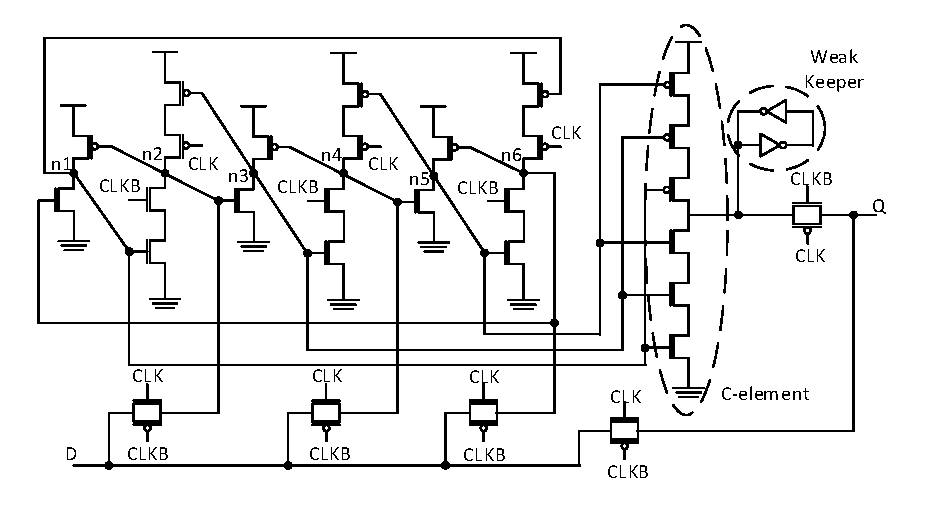
\includegraphics[trim = 0mm 6mm 0mm 4mm, clip, width=\linewidth]{Figures/HSMUF}
 %where an .eps filename suffix will be assumed under latex, 
 %and a .pdf suffix will be assumed for pdflatex; or what has been declared
 %via \DeclareGraphicsExtensions.
\caption{HSMUF latch \cite{HSMUF} with a weak keeper on the output.}
\label{HSMUF_fig}
\end{figure}
 
As stated previously, latches that are capable of recovering all nodes after an error are called robust. This unique feature is desirable since it leads to more efficient latch designs that can recover from an error when the latch is clock gated. The most efficient existing DNU-robust design is the DONUT (Double Node Upset Tolerant) latch proposed in \cite{DONUT} as shown if Fig. \ref{fig:DONUT}. This latch is based on the combination of four DICE latches creating twelve nodes. As in Fig. \ref{fig:DONUT}, each node is connected to multiple cross coupled elements. In the diagram, a cross-coupled element is denoted by a box with an arrow. The arrow gives the direction of the element from input to out. The pass gates are given below the design where \textit{D} represents the input to the latch and the given node number represents the node at which the pass-gate is connected.

Since the design is based on the DICE latch, it is able to exploit the recovery feature of the latch. One issue that was discovered during the testing of this latch is that it suffered from excessively high power and delay. It was found that the root of the problem was due to contention on the data loading lines. To solve this issue, the latch was modified such that the data loading nodes were set to high impedance during the transparent mode. As shown in Section \ref{sec:res}, this modification saved a large amount of power. This design is referred to as the DONUT-M and is given in Fig. \ref{DONUT_M}.

\begin{figure}[!htbp]
	\centering
	%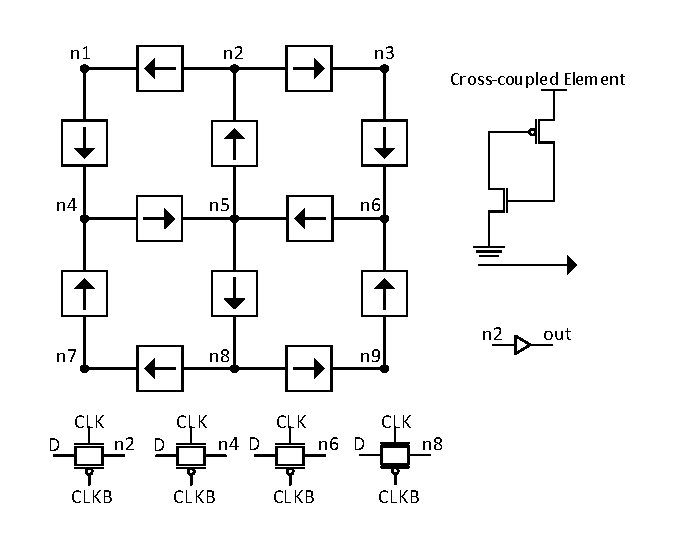
\includegraphics[width=\linewidth]{Figures/DONUT}
	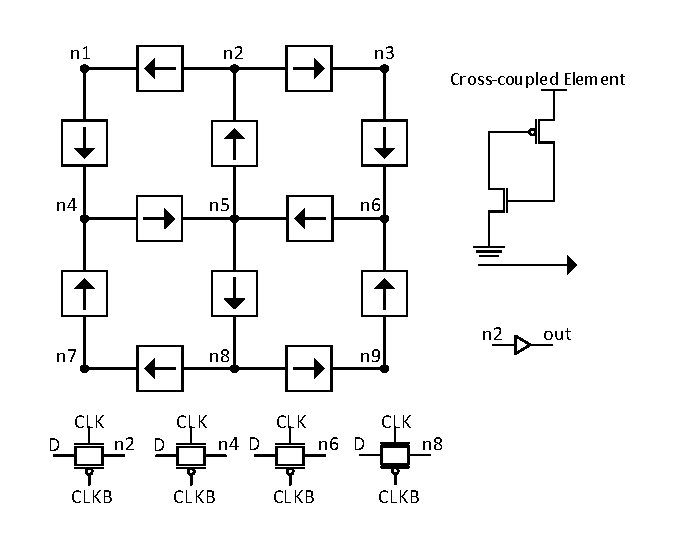
\includegraphics[trim = 0mm 12mm 0mm 7mm, clip, width=\linewidth]{Figures/DONUT}
	%where an .eps filename suffix will be assumed under latex, 
	%and a .pdf suffix will be assumed for pdflatex; or what has been declared
	%via \DeclareGraphicsExtensions.
	\caption{DONUT latch as proposed in \cite{DONUT}.}
	\label{fig:DONUT}
\end{figure}

\begin{figure}[!htbp]
	\centering
	%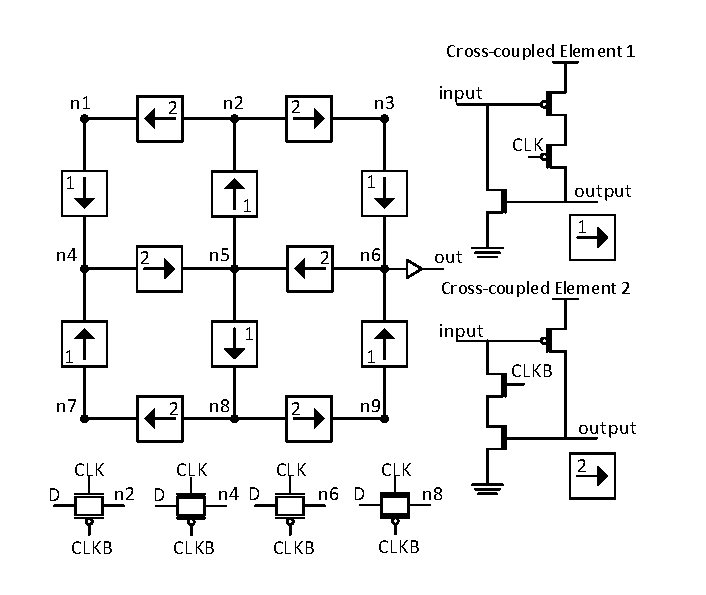
\includegraphics[width=\linewidth]{Figures/ModDONUT}
	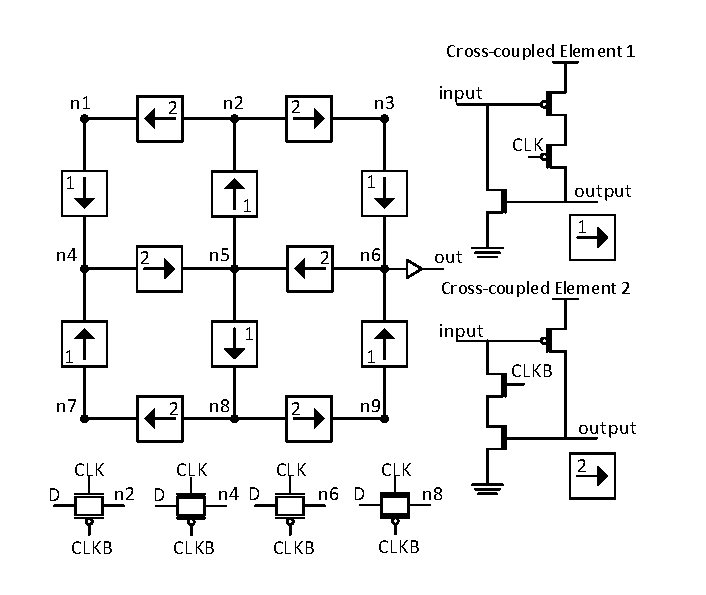
\includegraphics[trim = 0mm 5mm 0mm 7mm, clip, width=\linewidth]{Figures/ModDONUT}
	%where an .eps filename suffix will be assumed under latex, 
	%and a .pdf suffix will be assumed for pdflatex; or what has been declared
	%via \DeclareGraphicsExtensions.
	\caption{Modified low-power DONUT latch.}
	\label{DONUT_M}
\end{figure}

In addition to DNU tolerant latches, we also investigate the TNU latch. The authors in \cite{Blum2007} propose a latch design that shows limited TNU tolerance. Their design uses eight nodes and eight 2-input C-elements. There are four input signals which are each connected to the output of a C-element to load the data during the transparent mode. In the hold mode, the latch is fully tolerant to a DNU since at least one of the erroneous nodes will be driven by a C-element with error-free inputs. However, when a TNU occurs, the latch is only tolerant if all three errors are on adjacent nodes. 